\documentclass{beamer} %[handout]
%\usepackage{amsmath, amsfonts, amssymb}
\usepackage{natbib, apalike}
\usepackage[english,ngerman]{babel}
\usepackage[utf8x]{inputenc}				%fuer Umlaute
\usepackage[math]{iwona}
\usepackage[absolute,overlay]{textpos}		%fuer textblocks
\usepackage{wasysym} 					   %für verschiedene Sonderzeichen/Symbole
\usepackage[listings,theorems]{tcolorbox}	%fuer colorboxes
\usepackage{graphicx}
\usepackage{ifsym}
\usepackage{ulem}
\usepackage{xspace}
\usepackage{todonotes}
\usepackage{subfloat}

% Choose theme:
\usetheme{Amsterdam}

% MAKE PRESENTATION MORE PRETTY:
	%%remove navigation symbols
	\setbeamertemplate{navigation symbols}{}	
	%% avoid hyphenation:
	%\tolerance=1
	%\emergencystretch=\maxdimen
	%\hyphenpenalty=10000
	%\hbadness=10000
\setbeamertemplate{footline}[frame number]
%% Custom commands and definitions:
\newcommand{\wichtig}[1]{\large{}\colorbox{blue}{#1}\normal size{}}
\newcommand{\p}{\item}
\newcommand{\pf}{$\rightarrow$}
\definecolor{darkblue}{HTML}{300000}

% Define title page contents:
\title{Body size trends in Neogene tortoises}
\subtitle{\small Did tortoises evolve towards a smaller body size?}
\author{Julia Joos}
\institute[OS]{Humboldt-Universität zu Berlin}
\date{28.09.2017}
%\titlegraphic{\includegraphics[scale=0.35]{pics/hu.png}}


% HERE WE GO:
\begin{document}
%\nocite{*}

% Title page:
\begin{frame}[plain]
	\setcounter{framenumber}{0}
	\titlepage
\end{frame}


% Table of contents:	
%\begin{frame}[plain]
%	\tableofcontents
%\end{frame}

\section{Introduction}


\subsection{Body size trends in Neogene tortoises}

\begin{frame}{Terrestrial Tortoises}
\begin{picture}(300,250)
\put(0,90){
	%\missingfigure%\includegraphics[height=5 cm]{}
}
\put(150,210){
%\fbox{
\begin{minipage}[t]{0.5\linewidth}
\begin{itemize}[<+->]
\p 2 clades: Meiolaniidae \textbf{P}  and Testudinidae \textbf{P}
\p Meiolaniidae: extinct, used to be present in Australia + South America
\p Testudinidae: comprise all extant terrestrial tortoises (America, Europe, Africa, Asia)
\p Testudinidae: probably Asian origin, oldet fossils: North America + Europe
\p today's most famous examples: giant tortoises (Galapagos + Aldabra) --> \textbf{map?}
\p throughout Earth's history: many giant forms on the continents as well
\end{itemize}
\end{minipage}}
%}
\end{picture}
\end{frame}

\begin{frame}{Megafauna}
\begin{picture}(300,250)
\put(0,90){
	%\missingfigure%\includegraphics[height=5 cm]{}
}
\put(150,210){
	%\fbox{
	\begin{minipage}[t]{0.5\linewidth}
	\begin{itemize}[<+->]
	\p animals with body mass $>$ 44 kg = megafauna
	\p mammalian megafauna: popular, famous, well investgated
	\p megafauna extinctions! --> humans or climate change
	\p ...
	\end{itemize}
	\end{minipage}}
%}
\end{picture}
\end{frame}

\begin{frame}{Pleistocene Extinctions}
\begin{picture}(300,250)
\put(0,90){
	%\missingfigure%\includegraphics[height=5 cm]{}
}
\put(150,210){
	%\fbox{
	\begin{minipage}[t]{0.5\linewidth}
	\begin{itemize}[<+->]
	\p human influence
	\p climate change
	\p ...
	\p ...
	\end{itemize}
	\end{minipage}}

\end{picture}
\end{frame}

%overview at the end of the introduction!
\begin{frame}
\begin{enumerate}[<+->]
\p Body size distribution of Testudinidae?
\bigskip
\p Body size differences on spatial/temporal scale?
\bigskip
\p General body size trends?
%--> or rather continuous gene flow or all 3 species arose from one shared ancestor?
%\bigskip
%\p Reasons for extinction?
%\bigskip
%\textcolor{gray}{....}
\end{enumerate}
\end{frame}
%}
\section{Material \& Methods}

\subsection{Body size trends in Neogene tortoises}

%data set: how many, from which sources etc.
\begin{frame}{Data set}
%\begin{picture}(300,250)
%\put(170,80){
\begin{center}
	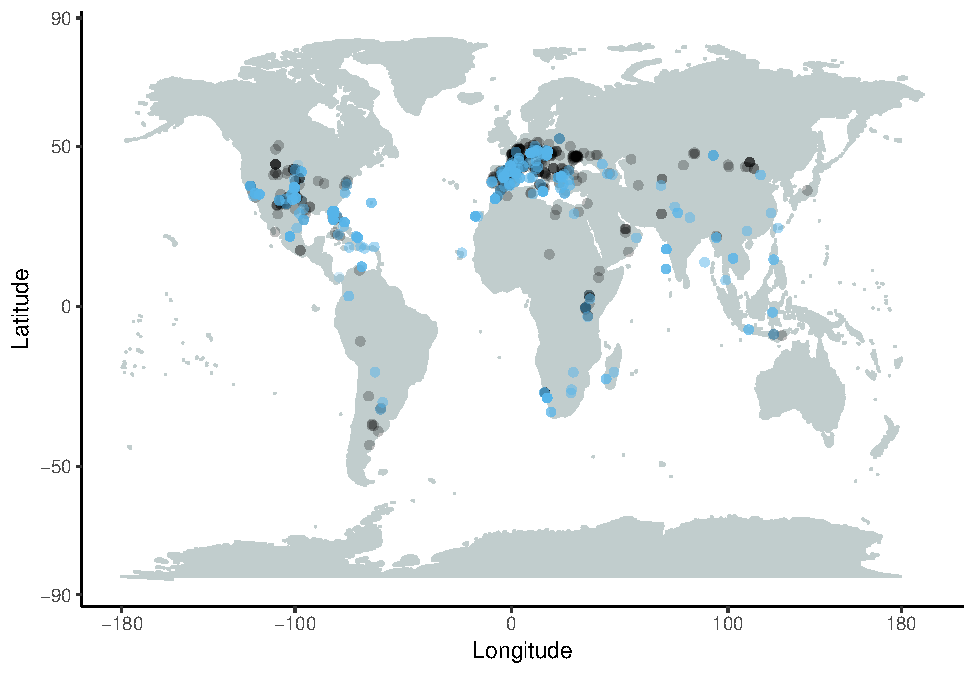
\includegraphics[width=0.7\textwidth]{MA_JJ_files/figure-latex/MapFossilOccurrences-1.pdf}
\end{center}

%\includegraphics[height=5 cm]<4-5>{pics/mm2.png}
%\includegraphics[height=5 cm]<6>{pics/mm3.png}
%\includegraphics[height=5 cm]<7->{pics/mm4.png}

%}
%\put(20,190){
%\fbox{
%\begin{minipage}[t]{0.5\linewidth}
\begin{itemize} %[<+->]
\p<1-> occurrences (black): 796 individuals, 647 localitis (Eocene - recent)
\bigskip
\p<2-> body size data (blue): 376 individuals, 193 localities (Miocene - recent)
\bigskip
\p<3-> of those: 106 from FosFarBase
\end{itemize}
%\end{minipage}}
%}

%\end{picture}
\end{frame}


% body size data: estimations etc.
\begin{frame}{Carapace length measurements/estimations}
%\begin{picture}(300,250)
%\put(170,80){
%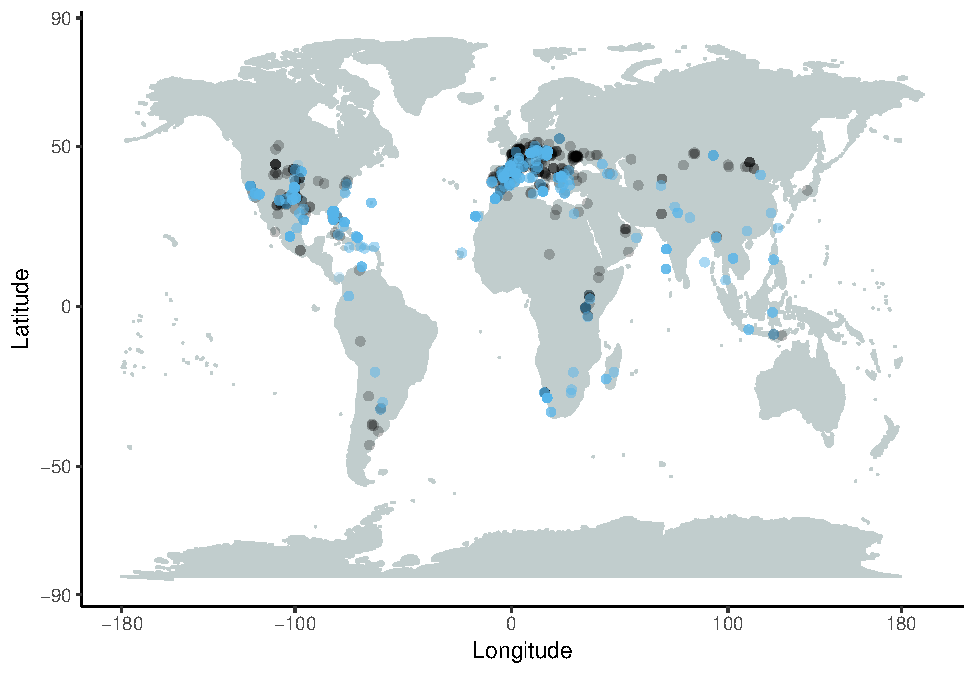
\includegraphics[width=0.7\textwidth]{MA_JJ_files/figure-latex/MapFossilOccurrences-1.pdf}
%\includegraphics[height=5 cm]<4-5>{pics/mm2.png}
%\includegraphics[height=5 cm]<6>{pics/mm3.png}
%\includegraphics[height=5 cm]<7->{pics/mm4.png}

%}
%\put(20,190){
%\fbox{
%\begin{minipage}[t]{0.5\linewidth}
\begin{itemize} %[<+->]
	\p<1-> exact measurements or estimations by original authors (n=...)
	\bigskip
	\p<2-> estimations from CL/PL ratio (--> extant measurements)
	\bigskip
	\p<3-> estimations from humeri/femora length, others (claw phalanges, verbal desription etc.)
\end{itemize}
%\end{minipage}}
%}

%\end{picture}
\end{frame}

% body size data: estimations etc.
\begin{frame}{Methods}
%\begin{picture}(300,250)
%\put(170,80){
%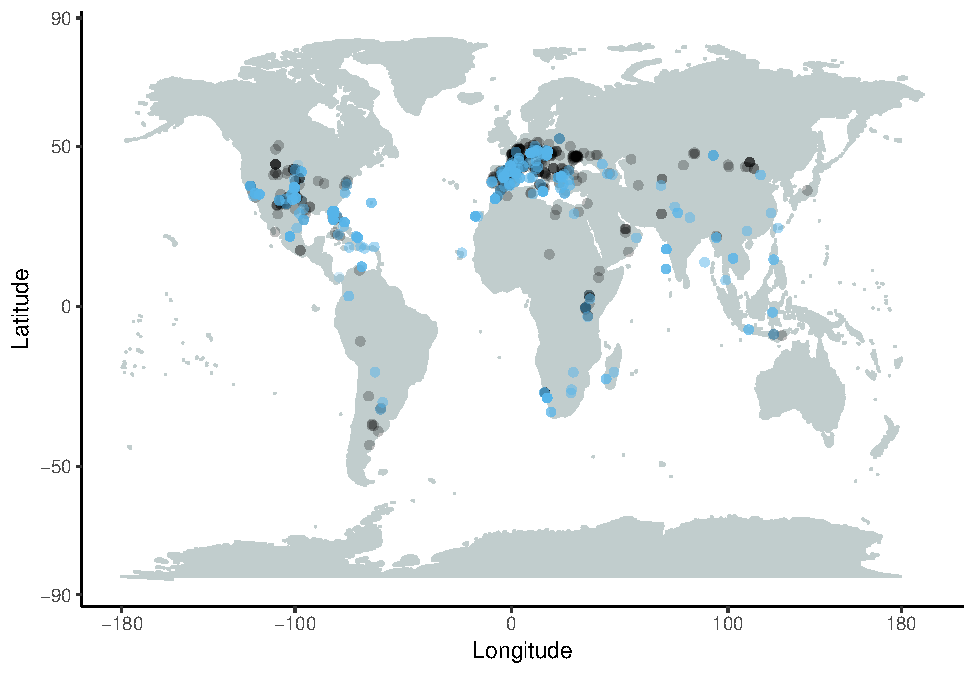
\includegraphics[width=0.7\textwidth]{MA_JJ_files/figure-latex/MapFossilOccurrences-1.pdf}
%\includegraphics[height=5 cm]<4-5>{pics/mm2.png}
%\includegraphics[height=5 cm]<6>{pics/mm3.png}
%\includegraphics[height=5 cm]<7->{pics/mm4.png}

%}
%\put(20,190){
%\fbox{
%\begin{minipage}[t]{0.5\linewidth}
\begin{itemize} %[<+->]
	\p<1-> SACs to check if sampling was sufficient --> generic level! add figure!!
	\bigskip
	\p<2-> histograms/density plots and boxplots (plus kruskal-wallis test, wilcoxon rank test)
	\bigskip
	\p<3-> paleoTS: fit different models to evolutionary trajectory of testudinid body size
\end{itemize}
%\end{minipage}}
%}

%\end{picture}
\end{frame}
\section{Body size distribution}


\subsection{Body size trends in Neogene tortoises}
%\subsection*{Genetic composition of alpine \protect\textit{Lycaeides} }

\begin{frame}
\begin{enumerate}
\p Body size distribution of Testudinidae?
\bigskip

\p \textcolor{gray}{
 Body size differences on spatial/temporal scale? 
%--> or rather continuous gene flow or all 3 species arose from one shared ancestor?
\bigskip
\p General body size trends? }
\end{enumerate}
\end{frame}


%Results1
\begin{frame}
Inhalt...
\end{frame}

%Discussion1


% % % % % % % % % % % % % % % % % % % % % % % % % % % % % % % % % % % % % % % % %

\section{Differences}
% on spatial/temporal scale


\begin{frame}
\begin{enumerate}
	
	\p \textcolor{gray}{Body size distribution of Testudinidae?}
	\bigskip
	\p Body size differences on spatial/temporal scale?
	%--> or rather continuous gene flow or all 3 species arose from one shared ancestor?
	\bigskip
	\p \textcolor{gray}{General body size trends?}
\end{enumerate}
\end{frame}




%Results2

%Discussion2




% % % % % % % % % % % % % % % % % % % % % % % % % % % % % % % % % % % % % % % % %
\section{Body size trends}

\begin{frame}
\begin{enumerate}
	
	\p \textcolor{gray}{Body size distribution of Testudinidae?
		\bigskip
		\p Body size differences on spatial/temporal scale? }
	%--> or rather continuous gene flow or all 3 species arose from one shared ancestor?
	\bigskip
	\p General body size trends?
\end{enumerate}
\end{frame}
%\include{Dis}
\section{Summary}

\subsection{Body size trends in Neogene tortoises}

\begin{frame}
\begin{enumerate}[<+->]
\p Body size distribution of Testudinidae?
\begin{itemize}
	\p[\pf] Bimodal distribution (left-skewed on islands!)
\end{itemize}
\p Body size differences on spatial/temporal scale?
\begin{itemize}
	\p[\pf] modern $<$ fossil
	\p[\pf] continental $<$ insular
\end{itemize}
\p General body size trends?
\begin{itemize}
	\p[\pf] stasis (generally and on islands)
	\p[\pf] URW (continental tortoises)
\end{itemize}

%\p Differences between men and women?

%\textcolor{gray}{....}
\end{enumerate}
\end{frame}





% CONTENT OF APPENDIX WON'T APPEAR IN THE HEADER. NUMBERING STOPS.
\appendix
\section[]{Backup}
\subsection[]{}

% First the references:
%\begin{frame}[noframenumbering]{Image sources}%[shrink=10]
%\begin{footnotesize}
%\begin{enumerate}
%\item ....
%\item ....
%\end{enumerate}
%\bibliographystyle{apalike}%ieeetr
%\bibliography{sea stars.bib}	% my bib-file
%\end{footnotesize}
%\end{frame}

%\newcounter{finalframe}
%\setcounter{finalframe}{\value{framenumber}}

\begin{frame}
\begin{center}
	Thank you!
\end{center}

\end{frame}

\end{document}